\documentclass[a4paper,xelatex,ja=standard,hiresbb,12pt]{bxjsarticle}
%各節を個別ファイルにする用
\usepackage{docmute} 
%設定ファイルは別に用意すると良い
\usepackage{zxjatype} 

\usepackage[a4paper]{geometry}	%A4サイズ
\geometry{left=25mm,right=25mm,top=20mm,bottom=25mm} %余白
\usepackage{setspace} %行間設定
\setstretch{1.5}
\usepackage[version=4]{mhchem} %化学式
\usepackage{here}
\usepackage{url}
\usepackage{lscape}
\usepackage{amsmath}
\usepackage{midpage}
\usepackage{exscale}

\usepackage{newtxtext,newtxmath} % Times系のフォントで英数字を表示する
\usepackage{xltxtra} % 游フォント好き...
\setCJKmainfont{游明朝 Regular}
\setCJKsansfont{游ゴシック Medium}
\setCJKmonofont{IPAGothic}

\bibliographystyle{IEEEtran} % 参考文献はIEEEの形式で入れる

\renewcommand{\figurename}{Fig.\,\,} % 図 1  じゃなくて Fig. 1 にしたかった
\renewcommand{\tablename}{Table\,\,} % 同上
\renewcommand{\thesection}{第\arabic{section}章} % ほんとは章じゃないけど

%ページ番号調節
\setcounter{page}{-3}

\begin{document}
%%%%%表紙%%%%%
\begin{flushleft}
\large{国際信州大学工学部 卒業論文}
\end{flushleft}
\vspace{150pt}
\begin{center}
        
\LARGE{hogeに向けたhoge導入に伴うhogeの\\hoge分析}
\vspace{130pt}
        
\Large{機械知能・航空工学科 hoge研究室} 
\vspace{15pt}
        

\Large{学籍番号 名前} \\ 
\vspace{15pt}
\large{(令和2年3月)}
        
\thispagestyle{empty}	%ページ番号非表示
        
\end{center}
%%%%%%%%%%%%%
%表紙の裏は白紙にしたい
\newpage
\mbox{}
\thispagestyle{empty}
\newpage
%%%%%目次%%%%%
\tableofcontents
\thispagestyle{empty}	%ページ番号非表示
%%%%%%%%%%%%%
%目次の裏も白紙にしたい
\newpage
\mbox{}
\thispagestyle{empty}
\newpage

%%%%%本文%%%%%
\documentclass[a4paper,xelatex,ja=standard,hiresbb,12pt]{bxjsarticle}

\usepackage{zxjatype} 

\usepackage[a4paper]{geometry}	%A4サイズ
\geometry{left=25mm,right=25mm,top=20mm,bottom=25mm} %余白
\usepackage{setspace} %行間設定
\setstretch{1.5}
\usepackage[version=4]{mhchem} %化学式
\usepackage{here}
\usepackage{url}
\usepackage{lscape}
\usepackage{amsmath}
\usepackage{midpage}
\usepackage{exscale}

\usepackage{newtxtext,newtxmath} % Times系のフォントで英数字を表示する
\usepackage{xltxtra} % 游フォント好き...
\setCJKmainfont{游明朝 Regular}
\setCJKsansfont{游ゴシック Medium}
\setCJKmonofont{IPAGothic}

\bibliographystyle{IEEEtran} % 参考文献はIEEEの形式で入れる

\renewcommand{\figurename}{Fig.\,\,} % 図 1  じゃなくて Fig. 1 にしたかった
\renewcommand{\tablename}{Table\,\,} % 同上
\renewcommand{\thesection}{第\arabic{section}章} % ほんとは章じゃないけど

\begin{document}
    \section{序論\label{sec:序論}}

    \subsection{研究目的}
    本研究ではhogeを対象にhogeを導入した際のhogeをhoge分析することで快感を得る.先行研究はこれ\cite{Hoge2025}.

    \subsection{本論文の構成}
    本論文では,hoge導入に伴うhogeeとhoge排出量増加を考慮したhoge分析を行う.本論文の構成は次のとおりである.\\
    \ref{sec:序論}は,序論である.\\
    \ref{sec:手法}では,hoge分析に用いるhogeの推計手法について述べる.\\
    \ref{sec:手法2}では,hoge分析の手法について述べる.\\
    \ref{sec:結果と考察}では,hogeの推計およびhoge分析の結果と考察を述べる.\\
    \ref{sec:結論}では,結論を述べる.

    \newpage
    

\end{document}
\clearpage
\documentclass[a4paper,xelatex,ja=standard,hiresbb,12pt]{bxjsarticle}

\usepackage{zxjatype} 

\usepackage[a4paper]{geometry}	%A4サイズ
\geometry{left=25mm,right=25mm,top=20mm,bottom=25mm} %余白
\usepackage{setspace} %行間設定
\setstretch{1.5}
\usepackage[version=4]{mhchem} %化学式
\usepackage{here}
\usepackage{url}
\usepackage{lscape}
\usepackage{amsmath}
\usepackage{midpage}
\usepackage{exscale}

\usepackage{newtxtext,newtxmath} % Times系のフォントで英数字を表示する
\usepackage{xltxtra} % 游フォント好き...
\setCJKmainfont{游明朝 Regular}
\setCJKsansfont{游ゴシック Medium}
\setCJKmonofont{IPAGothic}

\bibliographystyle{IEEEtran} % 参考文献はIEEEの形式で入れる

\renewcommand{\figurename}{Fig.\,\,} % 図 1  じゃなくて Fig. 1 にしたかった
\renewcommand{\tablename}{Table\,\,} % 同上
\renewcommand{\thesection}{第\arabic{section}章} % ほんとは章じゃないけど

\begin{document}
    \section{hogeの推計手法 \label{sec:手法}}
    hogeが開発したhogeをhogehogeすることでhogeを推計する.これは以下の式で表せる.
    \begin{equation}
        hoge = \sum_{hoge}^{hogehoge} Hoge
    \end{equation}
    %\bibliography{sotsuron}
    
\end{document}
\clearpage
\documentclass[a4paper,xelatex,ja=standard,hiresbb,12pt]{bxjsarticle}

\usepackage{zxjatype} 

\usepackage[a4paper]{geometry}	%A4サイズ
\geometry{left=25mm,right=25mm,top=20mm,bottom=25mm} %余白
\usepackage{setspace} %行間設定
\setstretch{1.5}
\usepackage[version=4]{mhchem} %化学式
\usepackage{here}
\usepackage{url}
\usepackage{lscape}
\usepackage{amsmath}
\usepackage{midpage}
\usepackage{exscale}

\usepackage{newtxtext,newtxmath} % Times系のフォントで英数字を表示する
\usepackage{xltxtra} % 游フォント好き...
\setCJKmainfont{游明朝 Regular}
\setCJKsansfont{游ゴシック Medium}
\setCJKmonofont{IPAGothic}

\bibliographystyle{IEEEtran} % 参考文献はIEEEの形式で入れる

\renewcommand{\figurename}{Fig.\,\,} % 図 1  じゃなくて Fig. 1 にしたかった
\renewcommand{\tablename}{Table\,\,} % 同上
\renewcommand{\thesection}{第\arabic{section}章} % ほんとは章じゃないけど

\begin{document}
    \section{hoge分析 \label{sec:手法2}}
    懲りずにhogeをhogeしてhoge分析を行う.
    

    %\bibliography{sotsuron}
\end{document}
\clearpage
\documentclass[a4paper,xelatex,ja=standard,hiresbb,12pt]{bxjsarticle}

\usepackage{zxjatype} 

\usepackage[a4paper]{geometry}	%A4サイズ
\geometry{left=25mm,right=25mm,top=20mm,bottom=25mm} %余白
\usepackage{setspace} %行間設定
\setstretch{1.5}
\usepackage[version=4]{mhchem} %化学式
\usepackage{here}
\usepackage{url}
\usepackage{lscape}
\usepackage{amsmath}
\usepackage{midpage}
\usepackage{exscale}

\usepackage{newtxtext,newtxmath} % Times系のフォントで英数字を表示する
\usepackage{xltxtra} % 游フォント好き...
\setCJKmainfont{游明朝 Regular}
\setCJKsansfont{游ゴシック Medium}
\setCJKmonofont{IPAGothic}

\bibliographystyle{IEEEtran} % 参考文献はIEEEの形式で入れる

\renewcommand{\figurename}{Fig.\,\,} % 図 1  じゃなくて Fig. 1 にしたかった
\renewcommand{\tablename}{Table\,\,} % 同上
\renewcommand{\thesection}{第\arabic{section}章} % ほんとは章じゃないけど

\begin{document}
    \section{分析結果と考察\label{sec:結果と考察}}
    \subsection{hogeの推計結果と考察}
    \ref{sec:手法}の手法で推計したhogeの結果をFig.\,\ref{fig:hoge推計結果}に示す.
        

    
    \begin{figure}[p]
        \centering
        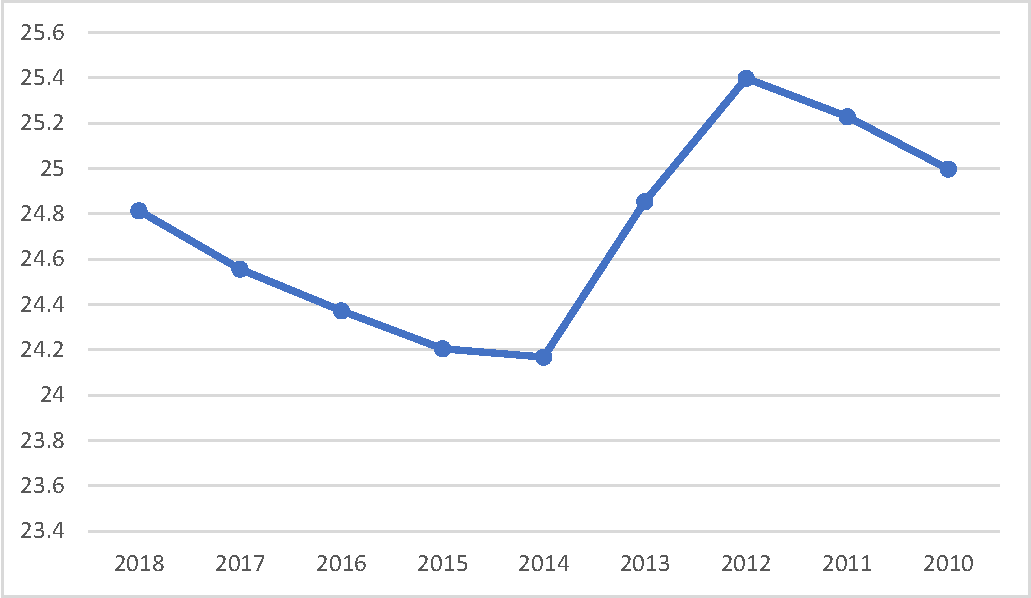
\includegraphics[scale = 0.7]{Figures/Hoge-crop.pdf}
        \caption{hogeの推計結果 \label{fig:hoge推計結果}}
    \end{figure}

    %\bibliography{sotsuron}
\end{document}
\clearpage
\documentclass[a4paper,xelatex,ja=standard,hiresbb,12pt]{bxjsarticle}

\usepackage{zxjatype} 

\usepackage[a4paper]{geometry}	%A4サイズ
\geometry{left=25mm,right=25mm,top=20mm,bottom=25mm} %余白
\usepackage{setspace} %行間設定
\setstretch{1.5}
\usepackage[version=4]{mhchem} %化学式
\usepackage{here}
\usepackage{url}
\usepackage{lscape}
\usepackage{amsmath}
\usepackage{midpage}
\usepackage{exscale}

\usepackage{newtxtext,newtxmath} % Times系のフォントで英数字を表示する
\usepackage{xltxtra} % 游フォント好き...
\setCJKmainfont{游明朝 Regular}
\setCJKsansfont{游ゴシック Medium}
\setCJKmonofont{IPAGothic}

\bibliographystyle{IEEEtran} % 参考文献はIEEEの形式で入れる

\renewcommand{\figurename}{Fig.\,\,} % 図 1  じゃなくて Fig. 1 にしたかった
\renewcommand{\tablename}{Table\,\,} % 同上
\renewcommand{\thesection}{第\arabic{section}章} % ほんとは章じゃないけど

\begin{document}
    \section{結論\label{sec:結論}}
    本研究では,いろいろやり,いろいろな結果が出た.その結果,いろいろなものがいろいろであることがわかった.めでたしめでたし.
\end{document}
\clearpage

%参考文献
\bibliography{sotsuron} 
\newpage
%これは謝辞
\documentclass[a4paper,xelatex,ja=standard,hiresbb,12pt]{bxjsarticle}

\usepackage{zxjatype} 

\usepackage[a4paper]{geometry}	%A4サイズ
\geometry{left=25mm,right=25mm,top=20mm,bottom=25mm} %余白
\usepackage{setspace} %行間設定
\setstretch{1.5}
\usepackage[version=4]{mhchem} %化学式
\usepackage{here}
\usepackage{url}
\usepackage{lscape}
\usepackage{amsmath}
\usepackage{midpage}
\usepackage{exscale}

\usepackage{newtxtext,newtxmath} % Times系のフォントで英数字を表示する
\usepackage{xltxtra} % 游フォント好き...
\setCJKmainfont{游明朝 Regular}
\setCJKsansfont{游ゴシック Medium}
\setCJKmonofont{IPAGothic}

\bibliographystyle{IEEEtran} % 参考文献はIEEEの形式で入れる

\renewcommand{\figurename}{Fig.\,\,} % 図 1  じゃなくて Fig. 1 にしたかった
\renewcommand{\tablename}{Table\,\,} % 同上
\renewcommand{\thesection}{第\arabic{section}章} % ほんとは章じゃないけど

\begin{document}
    \section*{謝辞}
    みんなありがとな
    
\end{document}

\end{document}